%! TEX root = ./master.tex
\lecture[Beweis von Seifert-van-Kampen. Berechunng der Fundamentalgruppe von Graphen]{Di 13 Jul 2021 12:12}{Beweis des Satzes von Seifert-van-Kampen}

\begin{remark*}
    An dieser Stelle haben wir nun den Beweis von \autoref{thm:seifert-van-kampen} gemacht. Aus zeitlichen Gründen ist der noch nicht aufgeschrieben, es fehlt aber auch \textit{nur} der Beweis, danach geht es normal weiter.
\end{remark*}


\begin{theorem}[allgemeine Version von Seifert-van-Kampen]\label{thm:seifert-van-kampen-allgemein}
    Sei $X$ ein Raum,  $x\in X$, und $\mathcal{U} = \left \{U_α\right\} _{α\in I}$ eine offene Überdeckung von $X$ mit  $x\in U_{α}$ für jedes $α\in I$. Sei für $α,β\in I$ stets $U_α \cap  U_β$ wegzusammenhängend. Die inklusionen
    \[
        \left \{ι_α\colon  \pi_1(U_α,x) \to  \pi_1(X,x)\right\}
    .\] 
    induzieren eine Abbildung
    \[
        \psi \colon  \coprod \pi_1(U_α, x) \twoheadrightarrow \pi_1(X,x)
    .\] 
    Dann gilt:
    \begin{enumerate}[1)]
        \item $\psi $ ist surjektiv.
        \item Falls darüber hinaus $U_α \cap  U_β \cap  U_γ$ wegzusammenhängend für $α,β,γ\in I$, dann ist der Kern von $\psi $ der Normalteiler erzeugt von
            \[
                \left \{ι_{α,β}(\omega ) ι_{β,α}(\omega )^{-1} \mid  \omega \in \pi_1(U_α \cap U_β, x), α,β\in I\right\} 
            .\] 
    \end{enumerate}
    wobei
    \begin{IEEEeqnarray*}{rCl}
        ι_{α,β}\colon  U_α \cap  U_β \hookrightarrow U_α \\
        ι_{β,α}\colon  U_β \cap  U_α \hookrightarrow U_β
    \end{IEEEeqnarray*}
    die Inklusionen sind.
\end{theorem}

\begin{oral}
    Man kann das im Wesentlichen aus dem üblichen Satz von \nameref{thm:seifert-van-kampen}   folgern, indem man induktiv auf endlich viele Mengen verallgemeinert. Für unendliche Mengen macht man dann ein Kolimes-Argument, indem man ausnutzt, dass wegen Kompaktheit jeder Weg und jede Homotopie schon in endlichen vielen der $U_i$ liegen muss.

    Für einen vollständigen Beweis siehe  \cite[Satz 1.20]{algebraic-topology-hatcher}.
\end{oral}

Wir werden diese allgemeine Version nicht beweisen, wir begnügen uns mit einigen Berechnungen.

\subsection{Berechnung der Fundamentalgruppe eines CW Komplexes}

\begin{theorem}[Graphen]\label{thm:fundamentalgruppe-von-graphen}
    Sei $X$ ein wegzusammenhängender Graph, und  $x_0\in X^0$, d.h.
    \[
    X = \underbrace{\bigcup_{i \in  I^0} e_i^0 }_{X^0} \cup \underbrace{\bigcup_{i \in  I^1} e_i^1
}_{1-\text{Zellen}} 
    .\]
    \begin{enumerate}[(i)]
        \item Es existiert $J\subset I^1$, so dass
            \[
            Y \coloneqq  X^0 \cup \bigcup_{j\in J} e_j^1
            .\] 
            ein maximaler \vocab{Baum} (ein zusammenziehbarer Graph, kombinatorisch: ein kreisfreier, zusammenhängender Graph) in $X$ ist. 
        \item Für $J$ wie in  $(i)$ gilt
             \[
                 \pi_1(X,x_0) \cong \coprod_{i\in I^1 \setminus J} \Z \cong \star_{i\in I^1 \setminus J} \Z
            .\] 
    \end{enumerate}
\end{theorem}

\begin{oral}
    Auch hier begnügen wir uns mit Beispielen, und führen keinen Beweis.
\end{oral}

\begin{example}
    \begin{itemize}
        \item 
    Betrachte folgenden Graph:
    \missingfigure{Graph mit Baum}
    der grün markierte Teilgraph ist nun ein Baum. Für die Berechnung der Fundamentalgruppe ziehen wir nun den Baum zusammen, also erhalten wir noch:
    \[
       X \simeq Y \coloneqq 
       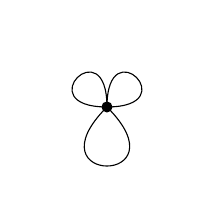
\begin{tikzpicture}[baseline = -0.2]
        \fill (0,0) circle (2pt);
        \draw (0,0) .. controls (1,0) and (0,1) .. (0,0);
        \draw (0,0) .. controls (0,1) and (-1,0) .. (0,0);
        \draw (0,0) .. controls (-1,-1) and (1,-1) .. (0,0);
    \end{tikzpicture}
\]
Der zusammengezogene Raum $Y$ ist dann tatsächlich homotop zum ursprünglichen Raum $X$, und  $Y$ ist nun frei mit so vielen Erzeugern, wie es Kanten in  $I^1 \setminus J$ gibt.
\item Betrachte  $Z$
    \[
    \begin{tikzcd}
        \arrow[loop left]{a} \ar{r}{b} x & y \ar[loop right]{c}
    \end{tikzcd}
\]
Dann ist $\pi_1(Z) = \left< α,β \mid  \right> $. Die Erzeuger sind gegeben durch $a, bcb^{-1}$
\item Ist $Z'$ der folgende Graph:
    \missingfigure{Graph}
    So sind die Erzeuger gegeben durch $a,bc b^{-1}, bd$
    \end{itemize}
\end{example}
